\usetikzlibrary{arrows.meta}
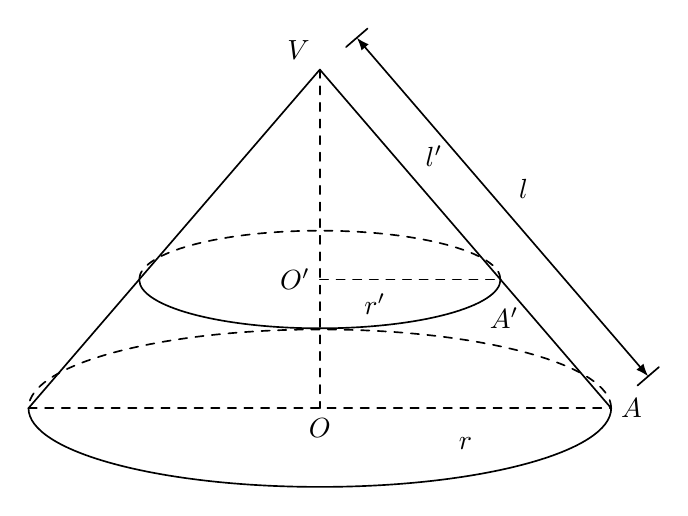
\begin{tikzpicture}[line width=0.6pt,line cap=round,line join=round]
\coordinate (V) at (0.0000,5.8000);
\coordinate (O) at (0.0000,1.5000);
\coordinate (A) at (3.7000,1.5000);
\coordinate (L) at (-3.7000,1.5000);
\coordinate (Op) at (0.0000,3.1340);
\coordinate (Ap) at (2.2940,3.1340);
\coordinate (Lp) at (-2.2940,3.1340);
\draw[dashed] (3.7000,1.5000) arc[start angle=0,end angle=180,x radius=3.7000,y radius=1.0000];
\draw (-3.7000,1.5000) arc[start angle=180,end angle=360,x radius=3.7000,y radius=1.0000];
\draw[dashed] (2.2940,3.1340) arc[start angle=0,end angle=180,x radius=2.2940,y radius=0.6200];
\draw (-2.2940,3.1340) arc[start angle=180,end angle=360,x radius=2.2940,y radius=0.6200];
\draw (V) -- (A);
\draw (V) -- (L);
\draw[dashed] (V) -- (O);
\draw[dashed] (L) -- (A);
\draw[dashed] (Op) -- (Ap);
\node[above left] at (V) {$V$};
\node[below] at (O) {$O$};
\node[left] at (Op) {$O'$};
\node[right] at (A) {$A$};
\node[xshift=0.00bp,yshift=-2.00bp] at (2.3400,2.7200) {$A'$};
\node at (1.8500,1.0500) {$r$};
\node at (0.7000,2.8200) {$r'$};
\node[inner sep=1pt] at (1.45,4.7) {$l'$};
\draw[{Latex[length=1.6mm]}-{Latex[length=1.6mm]},line width=0.6pt] (0.4700,6.2044) -- (4.1700,1.9044);
\draw (0.3335,6.0870) -- (0.6064,6.3218);
\draw (4.0335,1.7870) -- (4.3064,2.0218);
\node at (2.5853,4.2827) {$l$};
\end{tikzpicture}
